\subsection{Ejercicio 2}

Para representar el uso de 100 ciclos de CPU y dos tareas bloqueantes definimos el siguiente lote de tareas:\\

TaskCPU \\
TaskConsola 20 2 4\\
TaskConsola 25 2 4\\

TaskConsola realizará 20 y 25 llamadas bloqueantes respectivamente, con cada bloqueo de duración variable entre 2 y 4 ciclos. El cambio de contexto se fijo a 4 ciclos. En este ejercicio, el enunciado no aclaraba nada de costos de migración, con lo cual lo mantuvimos en cero. Estos fueron los gráficos obtenidos :



\begin{figure}[h]
  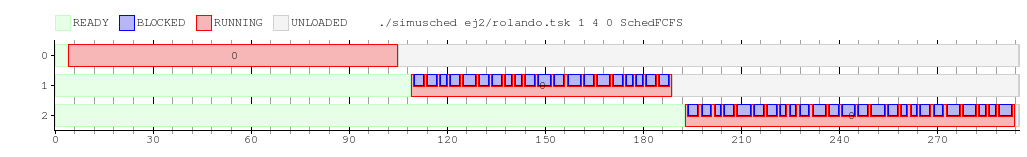
\includegraphics[width=\textwidth]{../ej2/uncore.png}
  \caption{}
\end{figure}

La latencia es el tiempo que un proceso tarda en empezar a ejecutarse. Con un núcleo, la latencia para las tareas será la suma entre el costo de cambio de contexto y la duración de la tarea anterior. En el caso de la primer tarea (la cero) su latencia es 4. La segunda tarea (la uno) tendrá latencia $ 4 + 100 + 4 = 108$. Por último, la tarea 2 tendra latencia $ 108 + duracion\_tarea1 + 4$.



\begin{figure}[h]
  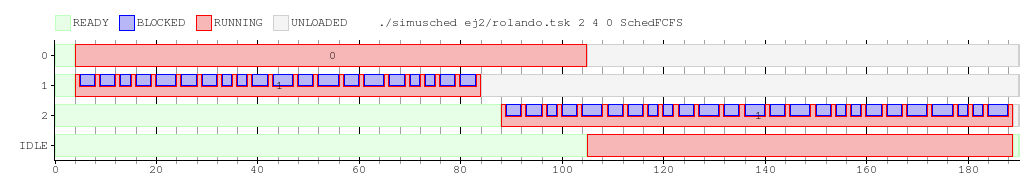
\includegraphics[width=\textwidth]{../ej2/doscores.png}
  \caption{}
\end{figure}

En cambio, con dos núcleos, la tarea cero tiene latencia 4, y las tareas uno y dos tienen 4 y duracion\_tarea1 + 4 respectivamente.

